\documentclass{../latex-setting/cmemoir}
\usepackage{scrextend}
\usepackage{minitoc}
\usepackage{shortvrb}
\usepackage{system-design} %Style For system-desing book


\begin{document}
\tableofcontents


\chapter{Web Crawler}


\begin{exercise}[Web Crawler Design Question/Summary:]
\begin{enumerate}
    \item What is a web crawler system? 
    \item Given some example in which internet is explored for specific purpose.
    \item How many pages will the crawler will process  approximalely? (reply: 1B per month)
    \item What do we need to store?
    
\end{enumerate}

\end{exercise}

\qicon What do we need to store?
\sicon HTML only for now.

\qicon How long we need to store the crawl result?
\sicon Lets assume we need to store 5year worth of data.



\newpage
\label{answers}
\begin{question}{What is a web crawler?}
   
    A web crawerl is a system that explores the word wide web (internet) to carry out specific task. Some of the examples what normall web-crawlers are used are:
    \begin{compactenum}[(i)]
        \item Index Generation for search gian like google,yahoo etc.
        \item Taking a time-snapshot of world wide web for archival or library purpose.
        \item Detect copyright infrignment.
        \item Detect sensitive code re-usage by anyone on the web.
        \item Extract specific images for modal training.
        \item etc \dots
    \end{compactenum}

\end{question}

\qq { What are the systems that gets involved in desinging a large application?}



\chapter{Web Crawler}

\qs{What is a web crawler?}
    A web crawler is a system that explores the internet with specific goal in mind. The goal can be be something like. (aka applicatio of web crawler)
    \ls
        \i Generate a snapshot of Internet at current time.
        \i Browse the internet for code duplicacy / piracy.
        \i Browse the web for search index generation for gians like Google Search.
        \i  Copyright Violation finding on document shared on internet.
        \i Research finding of something related to some search.
        \i download  all humans-dog interaction pics from instagram for ML modal training with the captions for machine modal traning.
    \le
\qe

\q{List Some Applications of web crawler.}


\ta{Design Considerations}
Now as we know what the system does, lets finilize what all feature we are required to implement from this system. Also, with what performace (latency, availibity, consistency) is expected from our system.

\lstart
    \i How many page download per month are we expecting? 
    \r{let's suppose it 1B per month.}
    
    \i Are we desiging for a single website (like school webcrawler to see suspicision activtiy from each user profile) or we are planning for whole web?
    \r{We are planning for whole web.}

    \i What is the document we are designing our crawler for?
    \r{For now lets just say we need HTML, but our system should be flexible to extend for other type also with minimum changes.}

    \i For how long do we need the downloaded data to be kept?
    \r{For our business purpose we need to store at maximum 5 years.}

    \i How about handling addition/deletion of a webpage?
    \r{You should consider newly added and edited pages too, you can ignore the page beign deleted.}

    \i Duplicate Content? How does the crawler respose to duplicate content?\marginnote{\small{As per data 23percentage content on internet is duplicat}}
    \r{Just ignore them.}

    Above are some of the sample question you can ask to clarify the system behaviour and working. This is a good time to be on same level as you and interview as what is expected from you to desing.
\lend

Besides above, there are many nonfunctional requirement of every system. They can vary from system to system (for example banking system need to be highly consistency, but that is not needed for chat server or photo storage, see \ref{chapter:cap} for more detials )

Going through types and problems of a distirbuted system, we find that our crawler system needs to be:
\ls
\i Highly Scalabile (scalability is required to extereme parallalization to handle billions of web pages.)
    Beside above this sytem also have extra non-functional requirement, which can be named as:
\i Robustness (The web is full of trap. Bad HTML, unresponsive server, malicions linke tec. The crawler must handle all these cases well without impacting the system)
\i Politines( The crawler should not make too many requirest to same host within short time interval)
\i Extensibility: our system should be flexible enough if we required to support other file type.
\le

\chapter{CAP in Districuted System}
\label{chapter:cap}

\qs{Types of System}
All the system can be categorirzed to some of the below: \\ 
(a) Highly Availalbe System / Strongly Availalbe System ex: \\
(b) Highly Consistely System / Strong Consistely system  ex: Banking system\\

\lstart
    \i System Scalibility
    \i System Availibility (should not slow down when the load is high, in extream case slow down means system stops responding)
    \i Tolerant System (System continue to work even though some part of the system is not working expected or are under heavy load)
\lend




\qe

System Reliability: Reliability refers to the ability of a system to consistently perform its intended functions without failures or errors over a specified period. It encompasses both availability and correctness.

System Resilience: Resilience refers to a system's ability to recover and adapt in the face of unexpected failures or disruptions. A resilient system can continue functioning even when individual components or parts fail.

System Redundancy: Redundancy involves duplicating critical components or resources in a system to ensure continued operation in case of failures. Redundancy can improve both availability and reliability.

Failover: Failover is the process of switching from a failed component or resource to a backup or redundant component to maintain uninterrupted service.

Load Balancing: Load balancing distributes incoming workloads across multiple resources to ensure even resource utilization, optimize performance, and prevent bottlenecks.

Scalability: As previously mentioned, scalability refers to a system's ability to handle increased workloads or demand by adding resources or adapting to changing requirements.

Performance: Performance relates to how efficiently a system responds to user interactions and processes tasks. High performance often involves minimizing response times and maximizing throughput.

Latency: Latency is the delay between initiating an action and receiving a response. Low latency is crucial for providing responsive and real-time services.

Throughput: Throughput measures the rate at which a system can process tasks or transactions. It indicates the system's capacity to handle a certain number of operations within a specific timeframe.

Bottleneck: A bottleneck is a point in a system where the flow of data or operations is restricted, leading to reduced overall performance.

Capacity Planning: Capacity planning involves estimating the required resources and infrastructure to meet current and future demands while maintaining performance and availability.

Elasticity: Elasticity refers to a system's ability to automatically and dynamically adjust its resources in response to changing workloads, helping to maintain performance and cost efficiency.

Distributed Systems: Distributed systems involve multiple interconnected components or nodes that work together to provide a unified service. Designing and managing distributed systems require considerations of consistency, availability, and fault tolerance.

Partition Tolerance: As part of the CAP theorem, partition tolerance refers to a system's ability to continue functioning in the presence of network partitions or communication failures between components.



\qs{CAP Theorme in Levels}
    (C) \b{Consistency Level:} Strong Consistency: In a strongly consistent system, all nodes in the distributed system see the same set of updates in the same order. Reads and writes are guaranteed to reflect the most recent write operation. Achieving strong consistency may require coordination and synchronization mechanisms, which can impact performance and availability, especially during network partitions.

    Eventual Consistency: In an eventually consistent system, updates made to the data will eventually be propagated to all replicas, but there is no guarantee about the order or timing of when different replicas will receive updates. Eventually consistent systems prioritize availability and partition tolerance over strong consistency. While eventual consistency can introduce short-lived inconsistencies, it often provides better availability and performance.
    
    Causal Consistency: Causal consistency ensures that operations that are causally related (where one operation depends on the result of another) are seen by all nodes in a specific order. Causal consistency maintains the causal relationship between operations while relaxing the requirement for global ordering of all operations.
    
    Read Your Writes Consistency: This level of consistency guarantees that if a client reads data after writing it, it will always see the write's effects. It provides a stronger guarantee than eventual consistency but doesn't necessarily ensure that other clients will see the effects of the write immediately.
    
    Monotonic Reads/Writes Consistency: These levels ensure that if a client reads or writes data multiple times, the reads/writes will not "go back in time." In other words, the data seen or written will be monotonically increasing.
    
    Bounded Staleness Consistency: This level allows for some lag in data synchronization between replicas. Data may be slightly stale, but the system guarantees that the staleness will not exceed a predefined bound.

    (A) \b{Availibility Levels:} High Availability (HA): High availability is a design principle that aims to ensure that a system remains operational and accessible with minimal downtime. HA systems often use redundancy, failover mechanisms, and load balancing to distribute traffic across multiple servers or instances. If one component or node fails, another can take over quickly to maintain service availability.

    Fault Tolerance: Fault-tolerant systems are designed to continue operating even when individual components or nodes experience failures. These systems employ redundancy, error detection and correction, and self-healing mechanisms to ensure continuous operation and data integrity.
    
    99.9per, 99.99per, 99.999per Availability: These percentages represent different levels of availability, often referred to as "nines." For example, "99.9per availability" means that the system is expected to be operational 99.9per of the time in a given period, leaving room for around 8.76 hours of downtime per year. Achieving higher availability percentages (more nines) requires more redundancy and fault-tolerant design.
    
    Distributed Denial of Service (DDoS) Mitigation: Many high-availability systems include DDoS mitigation strategies to protect against malicious attacks that could overwhelm a system's resources and lead to downtime.
    
    Recovery Time Objective (RTO) and Recovery Point Objective (RPO): These concepts are often used in disaster recovery planning. RTO refers to the maximum acceptable downtime following a failure, while RPO refers to the maximum acceptable data loss. Systems with high availability often have low RTO and RPO values.
    
    Redundancy and Failover: Highly available systems often use redundant components (such as servers, databases, and network links) and failover mechanisms to quickly switch to backup resources in case of a failure. This minimizes service disruption.
    
    Load Balancing: Load balancing distributes incoming network traffic across multiple servers or instances to ensure even utilization and prevent any single point of failure.
    
    Auto-Scaling: Cloud-based systems can automatically adjust their capacity based on demand. When traffic increases, the system can provision additional resources to handle the load, and scale down during periods of lower demand.
    
    Geographic Redundancy: Deploying resources across different geographic regions helps ensure availability even in the event of a regional outage or disaster.
    
    It's important to note that achieving high availability often involves trade-offs in terms of cost, complexity, and other factors. Organizations need to carefully balance their availability requirements with other considerations such as consistency, performance, and security.
    
    
    
    
    
    Regenerate
    

    (P) Partiotining Ways:
\qe
\chapter{Notification Sysyem}

\ha{Flow}
\ls
    \i What is a notification system?
    \i In which scenerio they are used? Give some common example then give.
    \i Give a example where user is notificed about its ticket confirmation later.
\le

\ha{About the System} 
A Notification system is a standalone system that is used to notify some short of events. It can be though as publisher and subscriber, publisher push the events to sent, and subscriber are those who are interested to these events.

Although this pub-sub modal works well with monolithich system, but for distributed system we need to take care of a lot of things.

\ha{Design Consideration and Solution/System Scope Finilization}

\ls

    \i Traffic: How many notificaion pe month we are targeting?
    \r{Lets suppose its 1B per month.}

    \i Notification Types and Target: Are we targeting for just SMS, or other types also like SMS,e-mail,PushNotification,NewsPaper Feed?
    \r{Lets say we need to support multiple ways, and our system should be extendable as if it can be supported easily for later addition/removal.}

    \i System Latency: How late is too much late?
    \r{Lets suppose that we need to have a latency of 2s, but is okay to deliver late if the system in under heavy load but no more than 60s late. \b{soft real-time system}}

    \i Notification Trigger: What triggers the notification?
    \r{Notifcation can be trigger when publisher publish any message. Or a job is completed or a manual sending try or any such similar things}

    \i Will user be able to opt-out?
    \r{definately}
\le



\ha{HLD Proposal}
Now, we know that we need a system that has publisher and substirubte to it. Lets try to propose a HLD, then we will imporove onto it.

Word Explanation: 
We will have a list of message publisher. These publisher will call our API to publish messages. We will provide a publisherServer for it. We will have a registrationServer which which sign-up upser and save their preference in database. It will also save registration info of publisher?. 

Once the publisherServer recieve a message from dispatcher. It will then analayis then, do dome property append if required and pass it to dispatcherQueue of appropriate type. (ex: a dispatcher want to send sms and email only). The front of the queue will be connected to a workerServer, which have a list of threads which will take the message in paraller from queue and forward it to \u{already exposed third party API for devices}.

\b{TODO: Now draw the digrama and explain work of each module and how they are connected. This completes the HLD}



\ha{LLD / Finding issue with system and proposing solution to fix it.}

\q{How to guarntee that message is delivered to device? aka Preventing Data Loss}
As this is a distributed system, it can happen that workerServer collapsed upon reasing the message. In this case how would be recover the system/\u{make sure message will reach the device}?

It can also happen that message is send to third-party, and third-party do not send ack to it?
\r{we can mark the message sent only if we recieve the ack from third-party server. This will also have a drawback that what will happen if server had sent the ack but it did not reach our server? => in this we have no option as to re-send the data. \marginnote{idempotent receiver}}

To mitigate worker crash issue, each worker can have logtable/logfile, which he will update status of message (like sending,sent,ack received) if it crashed, then he can re-read the logs and take appropriate decisions.

\hb{Notification Template}
Just like a word-template, we can have a notifcation template where the data can be populated for some field and then it is sent to user. By using this approach, we will have a less load on server and better design. We can later support pusblisher template also if they want their message to look different!

\hb{Notification Setting}
User would like to subscribe/re-subscribe and set daily notification setting etc. We need to provide user such facility. For this we will save user preferece in userDB. And during sending will check if user want the message or not.

\hb{Notification Analytics}
The manager would like to know if the message is read by user, clikced by user and time spent on reading, or similar analysits. We will collect all these data and save it to analyticsDB.
Start -> pening -> sent | error -> devlivered -> click | unsubscribed

\hb{Other Featurs}
Rate Limiting: to avoid overwheliming ujser with too many notification, we should limit the number of notification per hr. 

Retry Mechanics: When the third party faild to send notification, it will be queue in seperate retry queue. If the problem persist, then the developer is notificated via SMS or email.

Monitoring: Developer and Project Owner would like to via total number of queud notification. It is a important factor, and can be used to detect server load and Auto-Scaling if needed.

\ha{Summary}
TODO: Add summarization 
\chapter{News Feed System}

\ha{What is News Feed Systesm?}

A news feed is sytems that aggregate news/post/code other informatin from a set of post by other user/system. It thens shows them in desired order to the user. The system target is to provide information to the system user. One of the indirect goal of the system in to suggest content to user so that they will spend much of thier time on the web.

\hb{What the User can Post?}
User can post video,text,photo and other short info.


\hb{Real Life Use Case}
Some of the examples of system use are:
\ls
    \i Facebook News Feed System
    \i Instrgram Feed
    \i Google News Feed (data is generated from web itself)
    \i Twitter Timeline
\le

\ha{Design Scope Aggrement}
We will be asking question to decide how complex our system need to be. Also we will clarify any question regarding the system and performace and user expectatino.

\ha{Functional Features}
\lstart
    \i What the user is allowed to post?
    \r{user can post video,photo,text and external links}

    \i Can other user like,dislike ,post and comment on the post?
    \r{Yes, but its secondard to your explanation as main features will be post and timeline.}

    \i DAU? 
    \r{Lets suppose its 1B}

    \i Do we need storage?
    \r Yes, lets suppose we need storeage for 5 years.

    \i Are we designing mobile only app? web app? or both?
    \r Its both, giving user the flexibility to use the system at their convience.

\lend

\hb{Non Functional Features}
\lstart
    \i Its okay if uploading of a video takes a little time.
    \i Timeline generation should not take long,as it will user experience and user may leave the app.
    \i post of celebrity need to take special care.
    \i generation of timelint at runtime is expensigve, so we need to pre-compute it on our desing.
\lend

\ha{HLD Proposal}
Once we have basic understanding of the system, we can now propose initial desing. This way we can be sure that we and the interviewer agree on what is expected from the system.

There are two main featuers of our system (a) Post Services (b) Timeline Generation.

% TO-DO: Decrease pic resolution for fast compilation
    \b{HLD Diagram}\\
    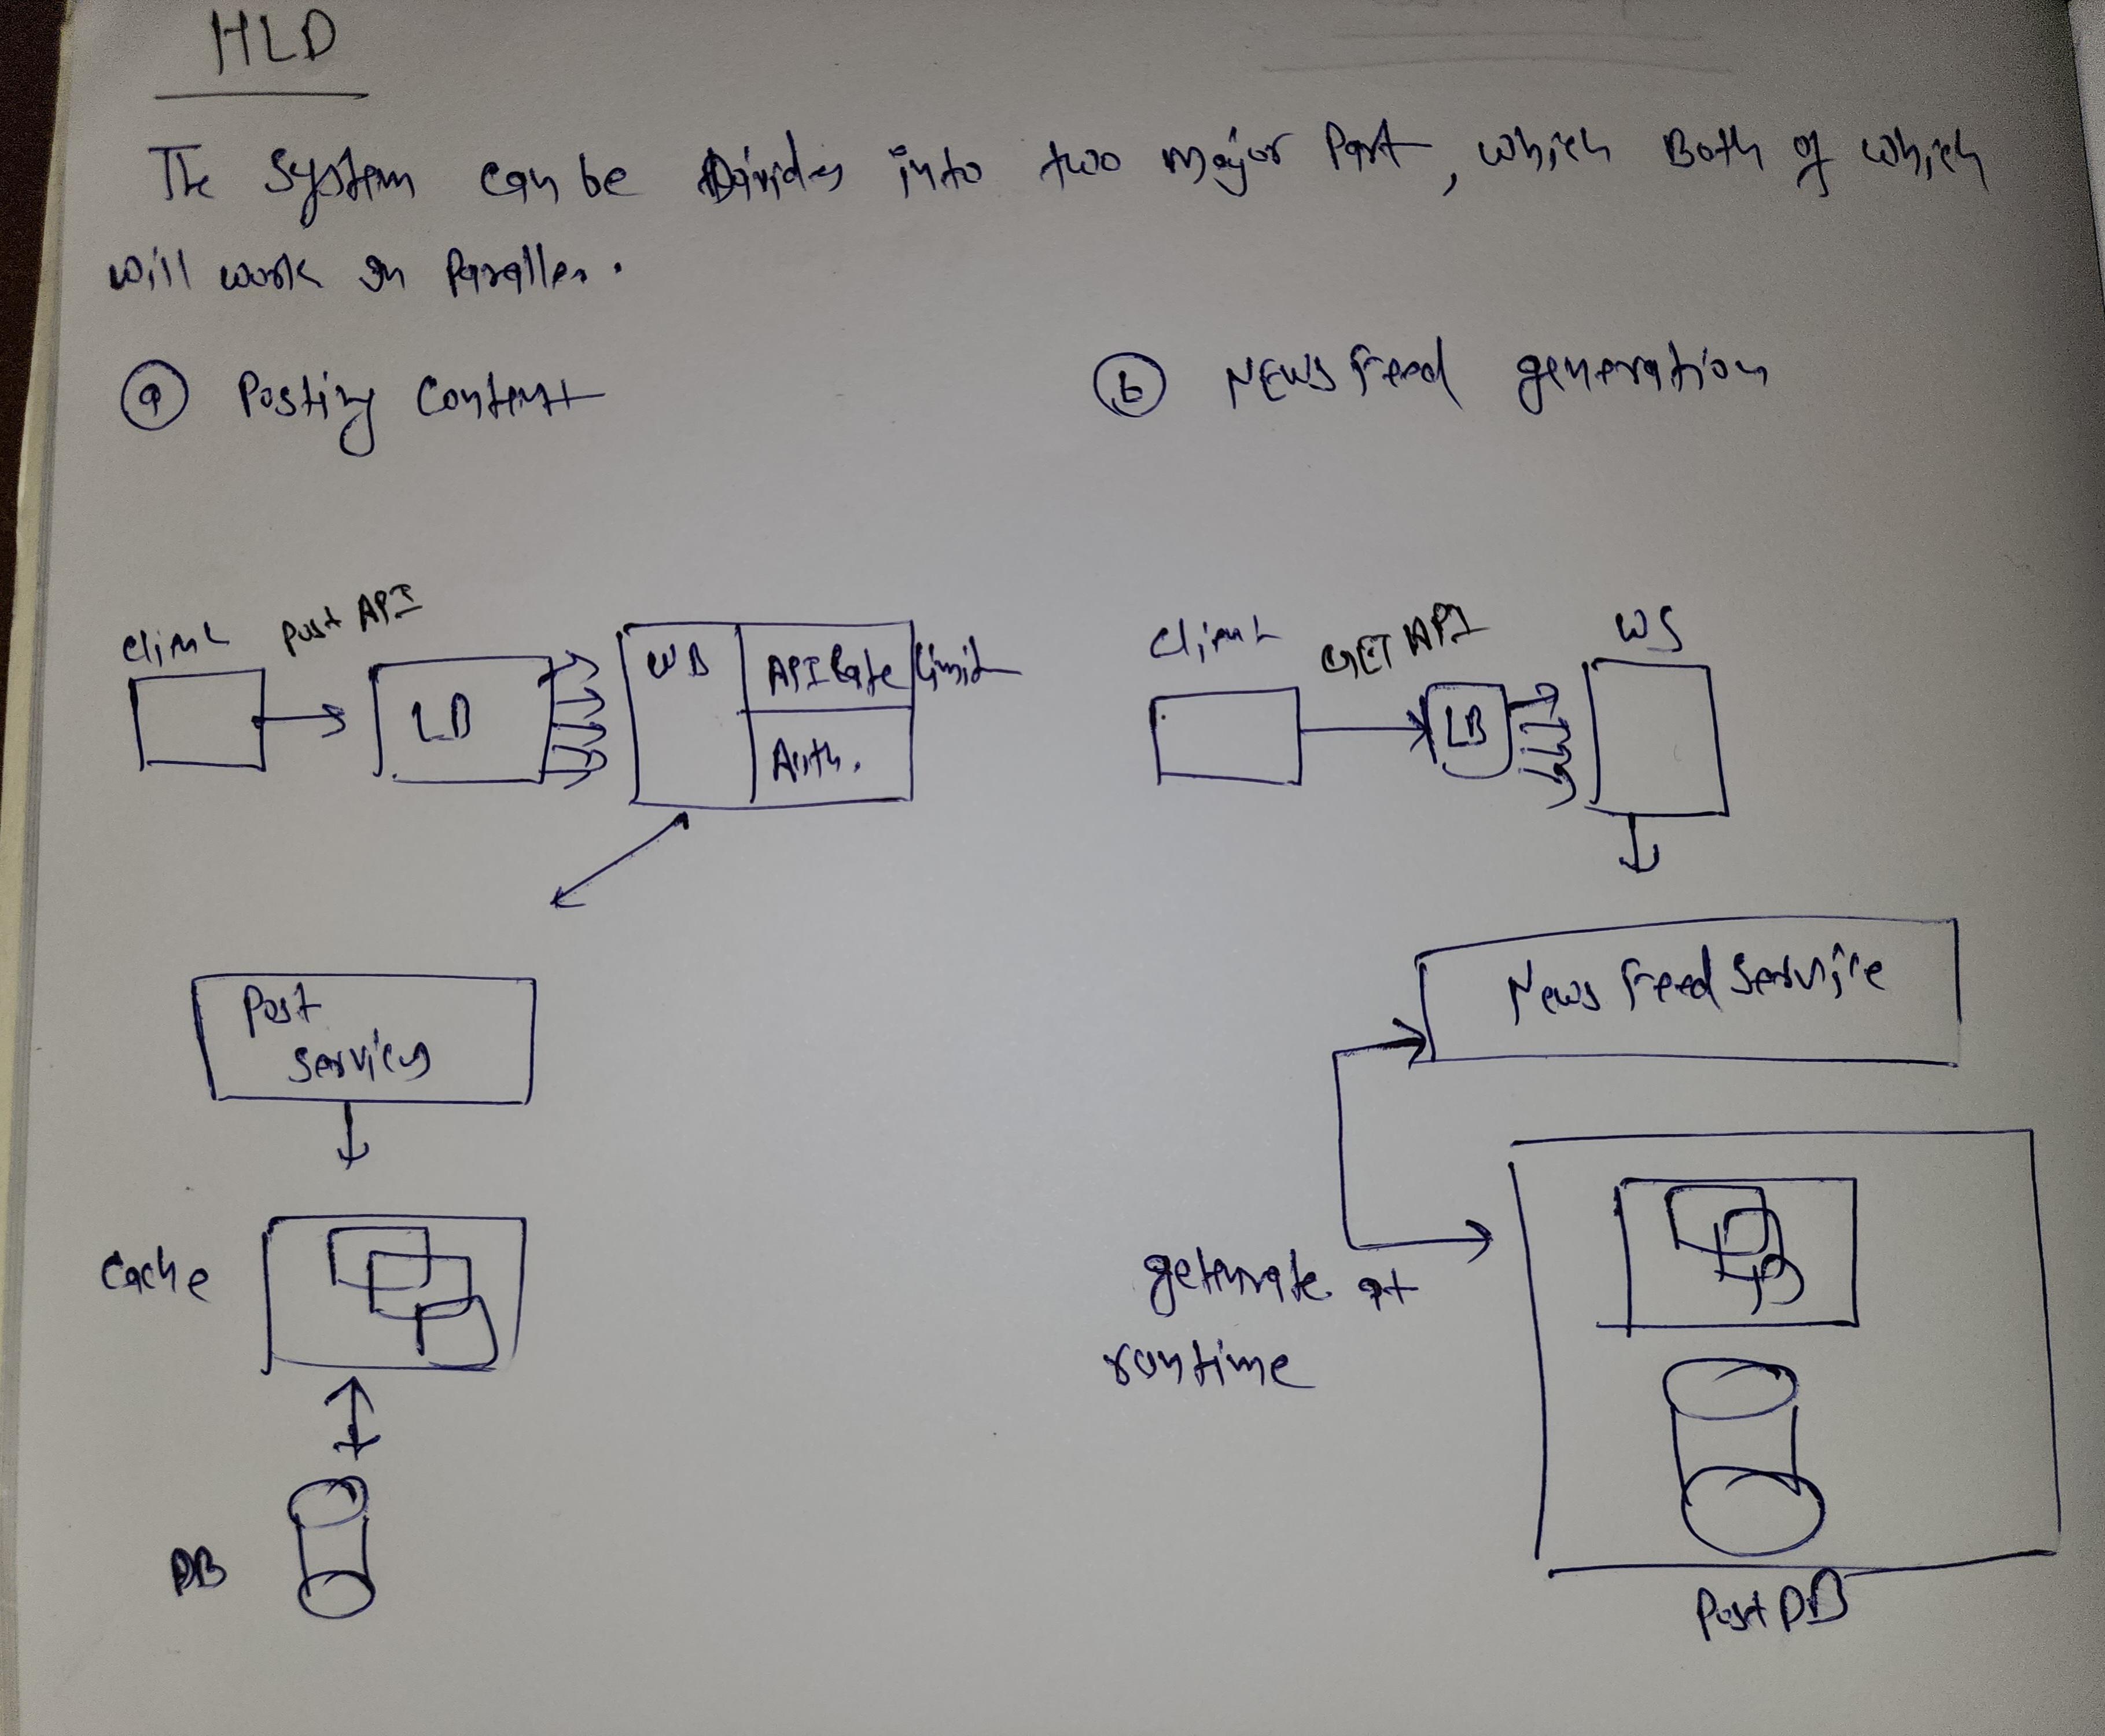
\includegraphics[width=0.7\textwidth]{resources/news-feed-hld.jpg}    



For posting, we will have our clients at either mobile/web. They will be post via exposed REST postAPI. They will be call the API and post the content. Once the webserver receives it forward the postrequest to postServices. It then save the data to DB, which is backed by cache.

For timeline generation, once the user opens the app then he will query the server. The server will check their friend list and their post,like etc and generate a JSON timeline response and send it to user.


\ha{HLD Evolution and LLD}
As we can observer there are various thing that make user experiance bad, and we can imporve them. Some of them are:
\lstart
    \i News Feed generation at run-time will take too much time. 
    \r We proposed alternative solution, in which news feed will be precomputed to save loading time on user time. Once any user post anything, then we pass that info to a new module called \u{Fanout Service}. The fanout service will get the user post and their friend list, and generate a (postID,userID) pair and push them into a queue. A set of worker thread keep reading this queue, it extracts a pair from the queue.And update userID timeline with consideration for the newly post. (if it want extra data it can query corresponding DB to get postDetails or userDetaisl.)

    \i With above approach, if the user has many friends / user the follow them. That that will lead to a heavy-increase in queue size, overall slowing the system. For these type of user, we will follow \u{Fanout on Read} instead of \u{Fanout On Write}. Once the user open their timeline, then recent post are pulled when user loads her homepage.

    \i For less-active user(who follows a celebrity), fanout on write works best. As computing resources are not waisted.

    \i How can we get list of friends?
    \r Instead of using SQL/No-SQl db, we use will be using \b{graphDB}  which works better with relationship data.

    \i Discuss userCache, postCache and newsFeedCache.
    \r These cases will be stored in front of DB, and instead of storing whole db-row, we will save metadata on the cache. (As original post is needed only if user loads the homepage, in all precomuption steps only their ID are sufficent.)

    \i Do we need CDN?
    \r Yes, as we know from socal media user want to see popular content. So if we place CDN also, static data load(like mangalyaan-3 landing) can be loaded fast.

    \i As we know we will need to be shard the userDB. Discuss the partiotioning strategy for best performace of the userDB and postDB.
\lend

\textbf{News Feed LLD}\\
\includegraphics[width=\textwidth]{resources/drawio/news-feed-lld.png}

\ha{Further Discussion Point}
As every system is complex, there will always be imporvement points. Some of the points can be applied to any system.
If time permits you can discuss and evolve the desing around these points alos:\

\hb{Scaling the DB}
\ls
    \i Vertical Scaling vs Horizontal Scaling
    \i SQL  vs No-SQL vs graphDB
    \i Master-Slave Replication and other replication strategy
    \i Read Replice and their use
    \i Consistely Models
    \i Databsse Sharding and avoiding common db problem like: hotspot problem
\le

\hb{Scaling the Desing}
\ls
    \i Keeping web tier stateless
    \i Caching and cache evicatioh policy and types of cache
    \i Use of multiple data center
    \i loose couple component with mesage queues
    \i Monitoring Features. (ex: QPS during peak hours, maximumm queue size etc)
    \i use of Notifcation system when post is generated.
\le


\chapter{Rate Limiter}

\ha{What is Rate Limter?}
A rate limiter is s system that limits the number of request that can be made to a system during a fixed time interval. It is used to controll incoming traffic or outgoing traffic. Server implement rate limiter to avoid overload of their system and avoid DDoS attack and better user experiance for majority of users.

In HTTP world, a rate limiter limits the number of client request allowed to be sent over a specified period. If the API request count exceeds the threshold defined by the rate limiter, all the excess calls are blocked.

\hb{Real World use case of rate limiting system.}
\lstart
    \i A user can write no more than 2 post per second.
    \i You can create a maximum of 10 accounts per day from same IP address.
    \i You can claim reward no more than 5 times per week from same device.
    \i Prevent resource starvation causes by DDoS attack.
    \i Reduce cost and cost approximation by reducing allowed request per minute.
    \i Allocating different API different priority  by assigining uneven timing to them.
\lend



\ha{Design Scope Discussion}

List of query that need to be finilized before starting the design.

\lstart
    \i It's a client side rate limiting or server side?
    \r Server Side.

    \i What are the parameter upon which the rate limiter will throttle the request? Is it IP address, userID or other properties?
    \r Let's say we want it to flexible.

    \i Number of calls to the Rate limiter?
    \r Lets say its 50M calls to the server upon which we want to intergrate the rate limiter.

    \i Is the system distriburted?
    \r Of Course.

    \i Do we need to inform the user that their request are beign throttled/dropped?
    \r Yes, a good system must not remain unambigous. We need to return 429 HTTP code in case the request get blocked due to rate limiting throttling. 
\lend

\hb{Non Funcitonal Requerement }
Here are some of the non functional requirement that we need to consider while desiging our system.

\lstart
    \i The system must not introduce significient latency. i.e it should be a \u{low latency} system, and should not slow down the HTTP request.
    
    \i Use minimum memory.
    \i  Exception Handling: return appropriate error-code upon different state.

    \i High Fault tolerance: If there is any problem with the rate limiter(ex: a cache servers goes offline), it should not affect the entire system.
\lend

\ha{Algorithms For Rate Limiting}

Where should the system be places?\\
It can be placed at API gateway or standalone version in between client and API server or can be buit inside of API server.

Rate Limting Algorithms.
\ls
    \i Token Bucket Algorithm.
    \i Leaking Bucket
    \i Fixed Widnow Counter
    \i Sliding Window long
    \i Sliding Window Counter
\le

Explain each of the above algorithms. In case of any query pleaser refer the book.


\ha{HLD Proposal}
Now as we understand the basic idea of rate limiting. It need to maintains a counter variable, and if the counter is above threshold then the subsequent request will be dropped. 

We need to pay attention that we are desigining a distributed system, so the counter will be incremented in a distributed way. 

Also the counter cannot be stored in disk as it will slow down the operation. So we will use in-memory data-store like redis, which is fast and provide distributed INCREMENT and EXPIRE operations. 
\marginnote{How redis prevent data-loss during system crash?}

\begin{lfigure}{resources/rate-limiter-hld.png}{0.5}{0.4}
    Rate limiter middleware is provided in between Client and API server. For every request, its corresponding count is checked from redis. If the count is above threshold then the request is dropped else it is allowed to pass to API server.
\end{lfigure}

\ha{LLD | Desing Deep Dive}
    In the desing deep dive, we will analyse the HLD for possible improvement and possible paint point which we must remove for a better system.

    \hb{ Distributed Rate Limiter | Solving Race Condition with minimum time:}
    As we know in a distributed system, the counter can be updated by tho threads in parallel. To avoid the race condition, one obivious solution is to use lock on the counter variable. \b{But it will slow down the system.}
    \rfl{Redis achieves atomicity by using a single-threaded architecture}
    In here, single type of operation is performed on single thread to avoid race condition entirely.

    \hb{Rate Limiting Rules(Storage,Actions):}
    We haven't answersed quesitions like:\\
     (a) How and rate limiting rules created and where are they stored?\\
     (b) How to handle request that are rate limited?

    (a) For First we can have a JSON structure that defines the rate limiter configuration. Its structure can be something like.
    \begin{code3}
        {
            domain:"messaing|auth",
            descriptors:
            {
                key:"message_type",
                value:"marketing",
                rate_limit_s:250s,
                request_per_unit:5
            }
        }
    \end{code3}

    This set of JSON will be stored in disk, and some worker thread can upload it to cache for fast access.

    (b) For second, we can add addition headers to the client response that descibes the system in full.
    \begin{code3}
        - X-Rate Limit-Remaining: The Remaning number of allowed request within the window.
        - X-Ratelimit-Limit
        - X-RateLimit-Retry-After
    \end{code3}

    
    \hb{Synchronization Issue}
    Again this problem will not arose in a single-thread architecture like redis.

   \begin{lfigure}{resources/rate-limiter-lld.png}{0.7}{0.28}
    Worker thread retrives the rules from disk and sotre them in cache. (cold cache?)
    
    Request beign dropped can be queue or dropped.
   \end{lfigure}

    \hb{Performance Optimization}
    Performance Optimization is common amoung distributed system. Some of the ways for optimizatioin for a distriburted system are: CDN, Cache, Multiple Data Center, Faster Algoritms, Alternater Desing, Decouple video decoupling via event queue, batch processing, precomputation for faster run-time tradeoff.
    
    In Rate limiter case, we must provide multiple-data-center, else request from far away user can reach a large time to reach the rate-limiter system itself. One best approach use it to provide rate-limiter to region at which the API server itself are placed.

    Along with it, during a sudden spike how can you change you alorithm that ensure that less number of site user experience system outage?

    Should we support a hard-limit or soft-limit? In soft limit the number of request are allowed to vary by say 10per.

    \hb{Monitoring}
    Monitoring metrix is must for fine tuning the rate limiter bandwidth. We can track QPS and other different factor, and we can take decision based on them.

    For example if rate limiting rules are too strict then relax them a bit. (rate limiting are too strict can be identified by the number of request being dropped per day.)
    
\ha{Further Discussion Points}
\ls
    \i Avoid Beign Rate Limited.
\le


\ha{Wrap Up}

Rate limiter system is good problem that shows how you can desing a simple system and intergrate with existing system. Rate limiter also show how to chose between different atomicity levels and Snapshot Isolation Levels.
\marginnote{See Data Intensive book for Atomicity Level and Isolation Levels}

Multple data center is must for such type of system. Algorithm selection and explaining their working is also a critical part of this system.

\todo{Summarize the chapter.}
\chapter{Design a Key Value Store}

\ha{What is a Key Value Store?}
A key value store in a distriburted system is a module that works as a distributed map.

\ha{Use Cases}
Distributed key-value shows how basics thing like CAP, replication, partiotioning,fault-torence, conflict resolution works in a distributed system.

\ha{Requirements}
\lstart
    \i key-value pair of size 10KB
    \i High availiblity: The system should response quickly, even during failure.
    \i High scalibity: The system should be scalable to support highter load in case the need arise.
    \i Server Addition and removal should take less time and consue less resources.
    \i tunable consistency via \u{quoram consenses}
\lend

\ha{Desing}

\hb{Single Server Store}
Discuss data compression to save space. cache for most used key and rest in disk.

Discuss why it cannot be used in distributed system and how scaling it is a challenging task.

\hb{Distributed Server Store}

Flow:
\lstart
    \i Discuss CAP theorem.
    \i Why partitions cannot be avoided in distributed system?
    
    \todo{Add fig of 3 system}
    If we chose consistency over availiblity(CP system),then we must block all write operation to n1 and n2 to avoid data inconsistency. (data inconsitecy amoungh these server can make the system unavailable)

    If we choose availability over consistency(AP System), then the system keep accepting reads,even though it might return stale data.

    Chosing the right CAP guarntees that the system will work according to designer requirements.

    Using quorum consensus we can fine tune consistency level.

    \vspace{0.7cm}
    Now you can continue discussing below system component.

    \i Data Partition 
    \i Data replication
    \i Consistency tuning | quorum consenses | consistency models
    \i Inconsistency Resolution | vector clock
    \i Handling failure | gossip protocol | sloppy quoram + Hinted Handoff | Merkle tree + anti-entryopy protocol 
    
    \vspace{0.5cm}
    \i system architecture diagram
    \i write path
    \i read path


\lend

\todo{add figure6-18}

\todo{add fig6-20, fig6-21}

Resouces:
\lstart
    \i https://bytebytego.com/
    \i Alex Xu Book 1
    \i ALex Xu Book2
    \i Grokking the system desing?
\lend


\end{document}